\documentclass{article}
\usepackage[ruled,vlined,linesnumbered]{algorithm2e}
\usepackage{algpseudocode}
\usepackage{amsmath}
\usepackage{amsthm}
\usepackage{graphicx}
\usepackage{subfigure}
\usepackage{float}
\usepackage{amsmath }
\usepackage{amsfonts }
\usepackage{pdfpages}
\usepackage{epsfig}
\usepackage{graphicx}
\usepackage{arydshln}
\usepackage{verbatim}
\usepackage{subfigure}
\usepackage{enumerate}
\usepackage{rotating}
\usepackage{threeparttable}
\usepackage{caption}
\usepackage{epsfig}
\usepackage{cite}
\usepackage{times}
\usepackage{geometry}
\usepackage{tikz}
\geometry{a4paper}
\usepackage[colorlinks,linkcolor=blue]{hyperref}
\begin{document}
	\title{AI3602 Data Mining Homework 1.1}
	\author{Kailing Wang 521030910356}
	\date{March 11.2024}
	\maketitle

	\section*{Question 1}
	A metric $d$ satisfies:
	\begin{enumerate}[1)]
		\item $d(i, j)\geq 0$
		\item $d(i, i) = 0$
		\item $d(i, j) = d(j, i)$
		\item $d(i, j) \leq d(i, k) + d(k, j)$.
	\end{enumerate}
	
	\begin{enumerate}[a.]
		\item The Jaccard distance is:
		$J(A, B) = 1 - \frac{|A \cap B|}{|A \cup B|}$. Suppose $A$ or $B$ is not empty, which is trivial. 
		\begin{enumerate}[1)]
			\item $|A \cap B| \leq |A \cup B|\neq 0$, $\frac{|A \cap B|}{|A \cup B|} \leq 1$: $J(A, B) \geq 0$.
			\item $\forall A, |A \cap A| = |A \cup A| = |A|$, $J(A, B) = 1-1 = 0$.
			\item $|A \cap B| = |B \cap A|, |A \cup B| = |B \cup A|$,
			
			$J(A, B) = 1 - \frac{|A \cap B|}{|A \cup B|} = 1 - \frac{|B \cap A|}{|B \cup A|} = J(B, A)$.
			\item To prove $J(A, B) \leq J(A, C) + J(C, B)$, this is:
			$$
			\frac{|A \cap C|}{|A \cup C|} + \frac{|C \cap B|}{|C \cup B|} \leq \frac{|A \cap B|}{|A \cup B|} + 1. 
			$$
			In the fig in \ref{tikz}, I represent each part of intersection. The inequality above can be written as
			\begin{center}
				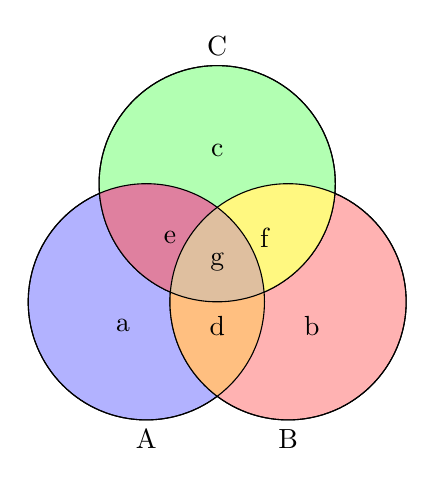
\begin{tikzpicture}[scale=1.5]
					\draw[fill=blue!30] (0,0) circle (1cm) node[below=1.5cm] {A};
					\draw[fill=red!30] (1.2,0) circle (1cm) node[below=1.5cm] {B};
					\draw[fill=green!30] (0.6,1) circle (1cm) node[above=1.5cm] {C};
					
					\begin{scope}
						\clip (0,0) circle (1cm);
						\fill[fill=orange!50] (1.2,0) circle (1cm);
					\end{scope}
					
					\begin{scope}
						\clip (0,0) circle (1cm);
						\fill[fill=purple!50] (0.6,1) circle (1cm);
					\end{scope}
					
					\begin{scope}
						\clip (1.2,0) circle (1cm);
						\fill[fill=yellow!50] (0.6,1) circle (1cm);
					\end{scope}
					
					\begin{scope}
						\clip (0,0) circle (1cm);
						\clip (1.2,0) circle (1cm);
						\fill[fill=brown!50] (0.6,1) circle (1cm);
					\end{scope}
					
					\draw (0,0) circle (1cm);
					\draw (1.2,0) circle (1cm);
					\draw (0.6,1) circle (1cm);
					
					\node at (-0.2,-0.2) {a};
					\node at (1.4,-0.2) {b};
					\node at (0.6,1.283) {c};
					\node at (0.6,-0.2) {d};
					\node at (0.2,0.5415) {e};
					\node at (1,0.5415) {f};
					\node at (0.6,0.333) {g};
					
				\end{tikzpicture}
				\label{tikz}
			\end{center}
			$$
			\frac{e+g}{a+c+d+e+f+g} + \frac{f+g}{b+c+d+e+f+g} - \frac{d+g}{a+b+d+e+f+g} - 1 \leq 0. 
			$$
			Use simpy to simplify the LHS to get $
				(- a^{2} b - a^{2} c - a^{2} d - a^{2} e - a b^{2} - 2 a b c - 4 a b d - 2 a b e - 2 a b f - 2 a b g - a c^{2} - 4 a c d - 2 a c e - 2 a c f - 2 a c g - 3 a d^{2} - 4 a d e - 3 a d f - 3 a d g - a e^{2} - a e f - a e g - b^{2} c - b^{2} d - b^{2} f - b c^{2} - 4 b c d - 2 b c e - 2 b c f - 2 b c g - 3 b d^{2} - 3 b d e - 4 b d f - 3 b d g - b e f - b f^{2} - b f g - 2 c^{2} d - c^{2} e - c^{2} f - 2 c^{2} g - 4 c d^{2} - 5 c d e - 5 c d f - 6 c d g - c e^{2} - 2 c e f - 3 c e g - c f^{2} - 3 c f g - 2 c g^{2} - 2 d^{3} - 4 d^{2} e - 4 d^{2} f - 4 d^{2} g - 2 d e^{2} - 4 d e f - 4 d e g - 2 d f^{2} - 4 d f g - 2 d g^{2})/D$, \\
			where $D$ is $\frac{1}{(a+c+d+e+f+g)(b+c+d+e+f+g)(a+b+d+e+f+g)}$, and we are really lucky to find the numerator already non-positive. 
		\end{enumerate}
		The Jaccard distance is a metric.
	
		\item 
		$\cos(\mathbf{a}, \mathbf{b}) = \frac{\mathbf{a} \cdot \mathbf{b}}{\|\mathbf{a}\| \|\mathbf{b}\|}$, simplified from the lecture PPT. 
		\begin{enumerate}[1)]
			\item Anyway, cosine distance is a cosine value within $[-1, 1]$, which is not non-negative.
		\end{enumerate}
		
		Cosine distance is not a metric. 
		\item 
		$$
		\text{levenshtein}(a, b) = \begin{cases}
			\max(i, j) & \text{if } \min(i, j) = 0,\\
			\min \begin{cases}
				\text{levenshtein}(a[1..i-1], b[1..j]) + 1\\
				\text{levenshtein}(a[1..i], b[1..j-1]) + 1\\
				\text{levenshtein}(a[1..i-1], b[1..j-1]) + 1_{(a_i \neq b_j)}
			\end{cases} & \text{otherwise}.
		\end{cases}
		$$
		It is hard to prove with pure equations. I'd use logical explanations. 
		\begin{enumerate}[1)]
			\item Obviously, according to definition, you can never edit a string negative times. 
			\item A string dose not need to be edited to get itself.
			\item You can inverse all the operations from string $a$ to $b$ to get $a$ from $b$. If in either direction the operation count is minimal, in the other direction it must also be minimal, i.e. is a levenshtein distance. 
			\item Proof by contradiction: If you can edit $a$ to $c$ and then to $b$ with less edit count than directly from $a$ to $b$, the route you found would replace the levenshtein distance path from $a$ to $b$ so this would never happen.
		\end{enumerate}
		The Levenshtein distance is a metric.
		
		\item
		$H(\mathbf{a}, \mathbf{b}) = \sum_{i=1}^{n} (a_i \neq b_i)$ 
		\begin{enumerate}[1)]
			\item A sum of bool is no way negative.
			\item The Hamming distance of a string with itself is always the 0 for it is the same as itself. 
			\item $(a_i \neq b_i)$ indicates $(b_i \neq a_i)$, which shows $H(\mathbf{a}, \mathbf{b})=H(\mathbf{b}, \mathbf{a})$.
			\item Here we derive a stronger conclusion:
			
			To prove $H(\mathbf{a}, \mathbf{b}) \leq H(\mathbf{a}, \mathbf{c})+H(\mathbf{c}, \mathbf{b})$, we'd prove
			$$\forall i \in [1, n], 1(a_i \neq b_i)\leq 1(a_i \neq c_i)+1(c_i \neq b_i):$$
			\begin{itemize}
				\item $a_i = b_i$, we have $1(a_i \neq c_i)+1(c_i \neq b_i) \geq 0=1(a_i \neq b_i)$.
				\item $a_i \neq b_i$, $c_i$ can be equal to at most one of $a_i$ and $b_i$, which is,
				$$2\geq1(a_i \neq c_i)+1(c_i \neq b_i) \geq 1=1(a_i \neq b_i)$$
			\end{itemize}
		\end{enumerate}
		The Hamming distance is a metric.
	\end{enumerate}
	Where is the lemma used? Confused. 
	
	
	\section*{Question 2}
	\begin{enumerate}[1.]
		\item Consider a uniform distribution inside a $L\times L$ square, the $x$ and $y$ coordinates of the position $p$ denote the the pair of the points in this problem. We are to calculate the expectation of $|x-y|$ inside the square:
		\begin{align*}
			\mathbb E [|x-y|] & = \int_0^L\int_0^L \frac{|x-y|}{L^2} dx dy \\
			& = 2 * \int_0^L\int_0^x \frac{x-y}{L^2} dx dy \\
			& = 2 * \int_0^L \frac{x^2}{2L^2}dx \\
			& = 2*\frac{L^3}{6L^2} = \frac{L}{3}
		\end{align*}
		\item $\mathbb E [||x-y||_2^2] = \mathbb E [\sum_1^d |x_i - y_i|^2] $, and since the coordinates distributed uniformly in all dimensions, 
		\begin{align*}
			\mathbb E [ |x_i - y_i|_2^2] & = \sum_1^d \mathbb E [ |x_i - y_i|^2] \\
			& = d \cdot \int_0^L\int_0^L \frac{|x-y|^2}{L^2} dx dy \\
			& = \frac{L^2d}{6}
		\end{align*}
		\item The possible range of the minimum distance $M$ is $[0, \frac{L}{N-1}]$. It's not easy to directly derive the probability of $M$. The distribution of all the points lie in an $N$ dimensional cube with volume $L^N$. It's easier to imagine the case when $M$ is larger than a certain $m$. Let ${x_n}$ be sorted, i.e. $x_1\leq x_2\dots \leq x_n$. This adds a probability scale $A_N^N=N!$. $P(M>m)$ shows $x_i + m < x_{i+1}, \forall i \in [1, N-1]$. This operation causes the high-dimensional cube to collapse, reducing $m$ on each axis. The length of the cube become $L - (N-1)m$. Note that this collapse dose not require the points to be sorted. To align the probability, we need to scale it by $\frac{1}{N!}$. 
		
		The probability $P(M>m)$ is thus given by $\frac{(L - (N-1)m)^N}{L^N}$.
		
		The expectation can be calculated by:
		\begin{align*}
			P(M) & = \int_0^{\frac{L}{n-1}}P(M>m)dm \\
			& = \int_0^{\frac{L}{n-1}} \frac{(L - (N-1)m)^N}{L^N} dm \\
			& =  - \frac{1}{N-1}\cdot\frac{1}{L^N} \cdot \frac{(L-(N-1)m)^{N+1}}{N+1} \bigg|_{0}^{\frac{L}{N-1}} \\
			& = \frac{L}{N^2-1}
		\end{align*}
		\item I don't really understand what the problem is asking. But since there is a minimum distance that is relatively low when $N$ is large, it is efficient to use $KD-tree$ with a certain neighbour range based on $P(M)$ when clustering. 
	\end{enumerate}
	\section*{Original Questions}
	\begin{figure}[ht]
		\centering
		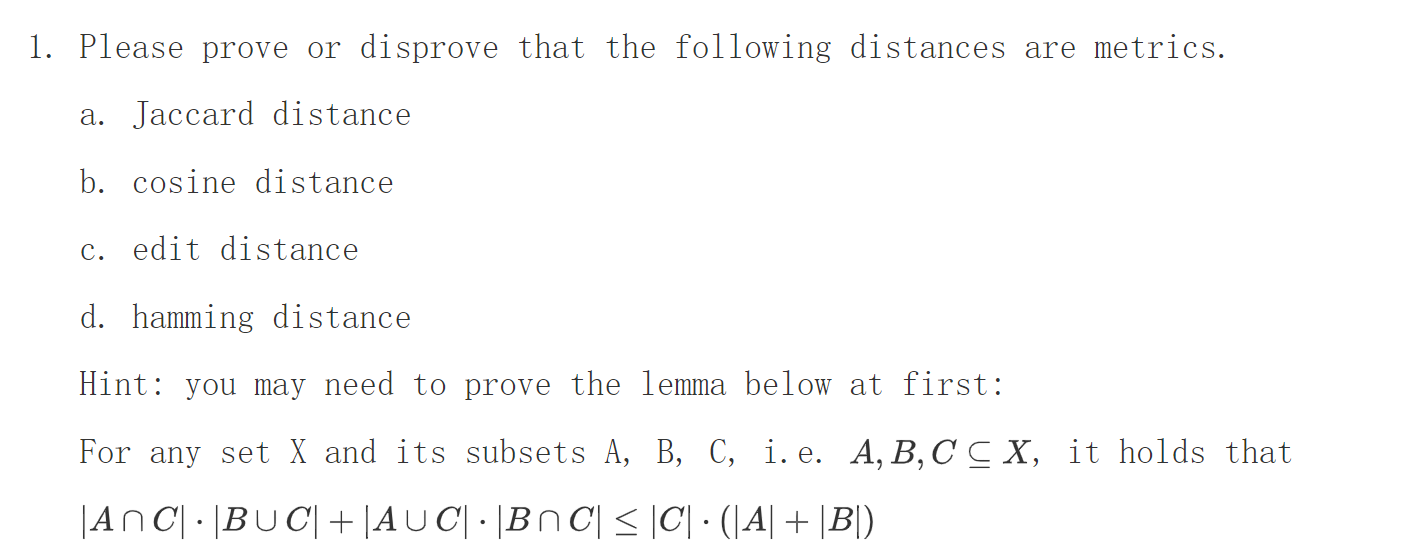
\includegraphics[width=0.8\textwidth]{q1}
		\caption{Question 1}
		\label{fig:1}
	\end{figure}
	\begin{figure}[ht]
		\centering
		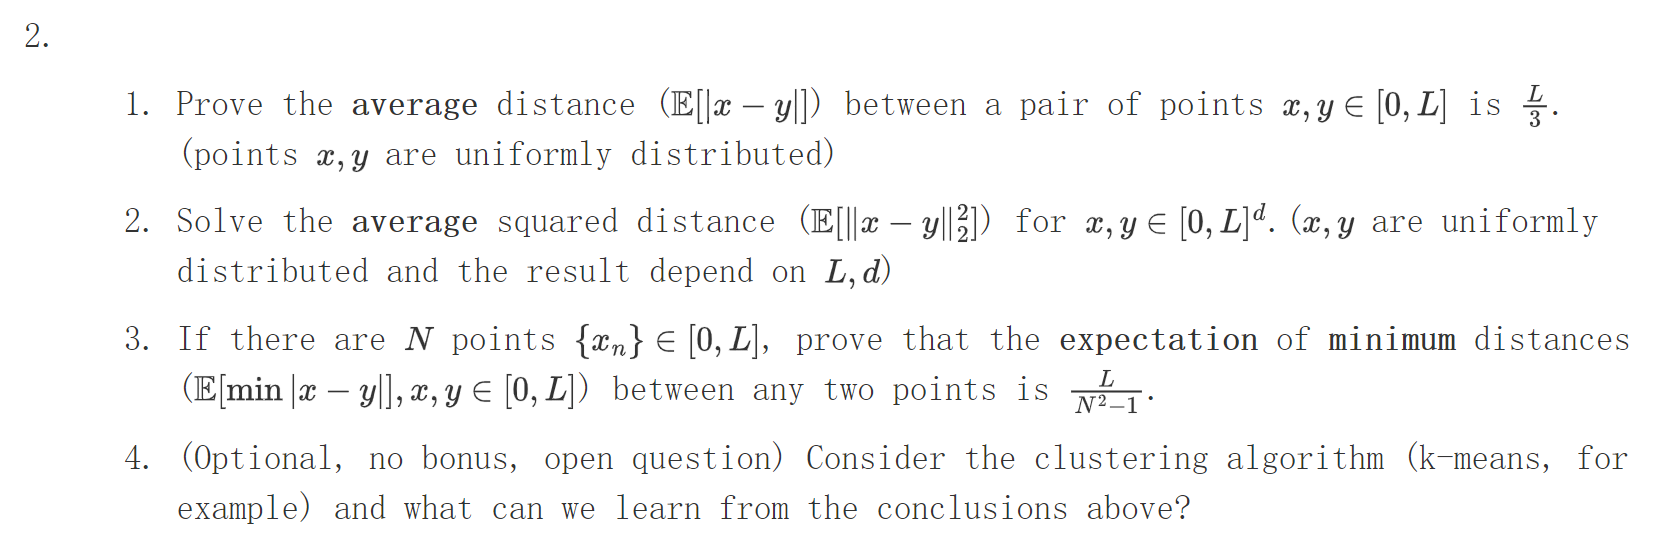
\includegraphics[width=0.8\textwidth]{q2}
		\caption{Question 2}
		\label{fig:2}
	\end{figure}
	\section*{Reference}
	\href{https://math.stackexchange.com/questions/1999612/average-minimum-distance-between-n-points-generate-i-i-d-with-uniform-dist}{stackexchange}
	
	\noindent Finished other parts independently with help of GPT only with the tikz image.
\end{document}
